\documentclass[10pt]{beamer}
\usepackage[utf8]{inputenc}
\usepackage{hyperref}
\hypersetup{colorlinks=true,linkbordercolor=blue,linkcolor=white,urlcolor=blue,pdfborderstyle={/S/U/W 1}}

\usepackage[scaled]{helvet}
\usepackage[T1]{fontenc}
\usetheme{Berkeley}
\beamertemplatenavigationsymbolsempty
\setbeamertemplate{headline}{}
\setbeamersize{sidebar width left=1.5cm}
\setbeamerfont{section in sidebar}{size=\fontsize{6}{6}\selectfont}
\setbeamerfont{title in sidebar}{size=\fontsize{6}{6}\selectfont}
\title{Tracing Backward Template}
\date{}

\begin{document}
\maketitle

\section{Topics}
\begin{frame}
\leftskip1em\textbf{Learn}
	\begin{itemize}
		\item to export and to complete a pre-filled Tracing Backward Template
	\end{itemize}
\vspace*{\fill}
Note: You need data from the tutorial \textcolor{blue}{\underline{\href{https://foodrisklabs.bfr.bund.de/data-collection-and-import/}{``Data collection and import''}}}. Please do this tutorial first.
\end{frame}

\section{1}
\begin{frame}
	\begin{center}
			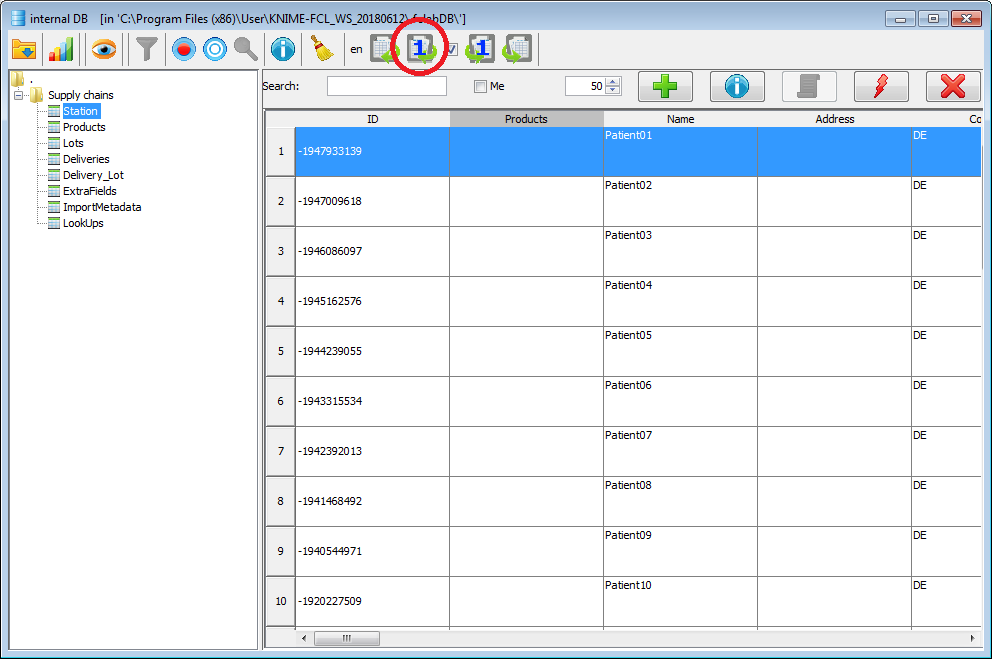
\includegraphics[height=0.6\textheight]{1.png}
	\end{center}
	\begin{itemize}
		\item Open the database and generate a Tracing Backward Template for a specific station, namely for \textit{Dry Stuff Inc}.
	\end{itemize}
\end{frame}

\section{2}
\begin{frame}
	\begin{center}
			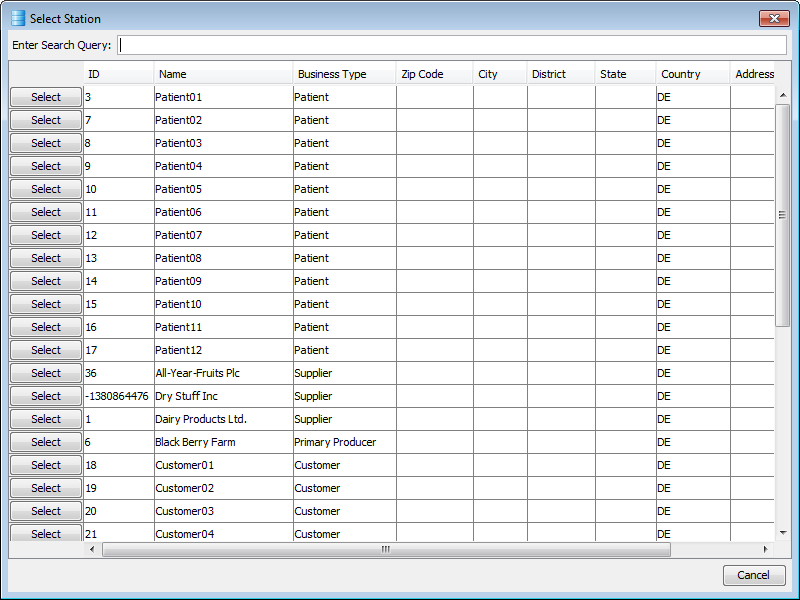
\includegraphics[height=0.6\textheight]{2.png}
	\end{center}
	\begin{itemize}
		\item Start typing ``dry'' and then click the ``Select'' button on the left.
		\item Choose a folder to save your pre-filled Tracing Backward Template.
	\end{itemize}
\end{frame}

\section{3}
\begin{frame}
	\begin{center}
			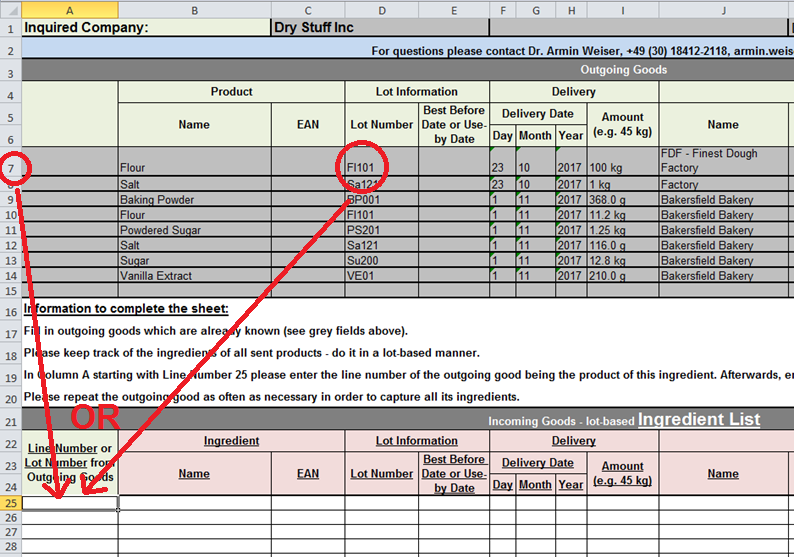
\includegraphics[height=0.6\textheight]{3.png}
	\end{center}
	\begin{itemize}
		\item Fill in the data from \textcolor{blue}{\underline{\href{https://github.com/SiLeBAT/BfROpenLabResources/raw/master/GitHubPages/documents/FCL\_Tracing\_backward\_template/Dry-Stuff-Inc.docx}{``Dry-Stuff-Inc.docx''}}}.
		\item Please make sure that you write the corresponding Excel row OR the corresponding lot number into column A to tell the database, that the ingredients went into a specific outgoing good.
	\end{itemize}
\end{frame}

\section{4}
\begin{frame}
	\begin{center}
			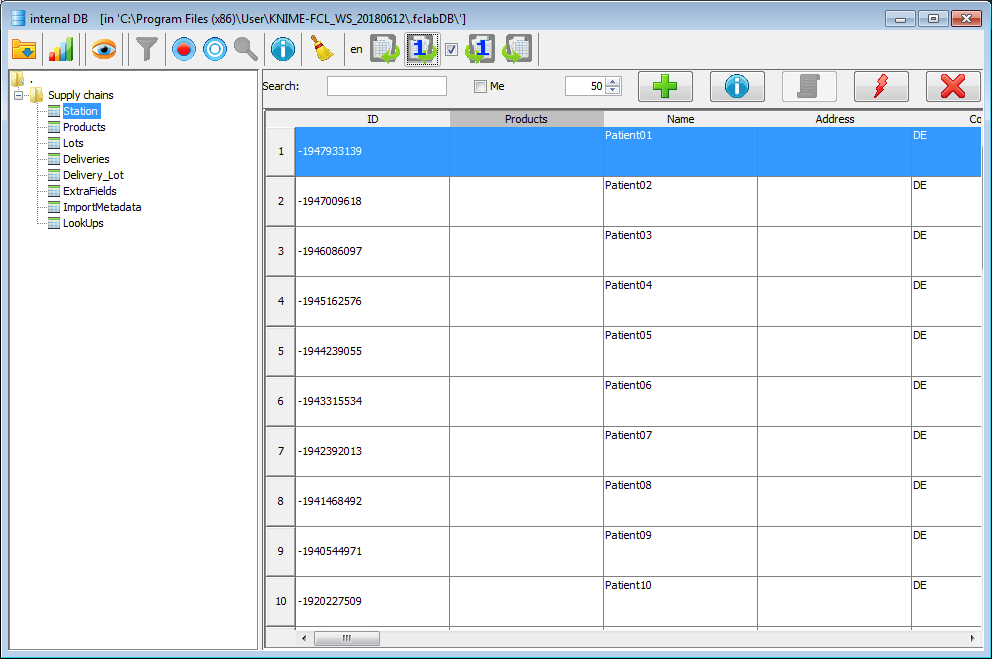
\includegraphics[height=0.6\textheight]{4.png}
	\end{center}
\leftskip1em{In KNIME:}
	\begin{itemize}
		\item Import your file into the database (see import button in the red circle).
	\end{itemize}
\end{frame}

\section{5}
\begin{frame}
	\begin{center}
			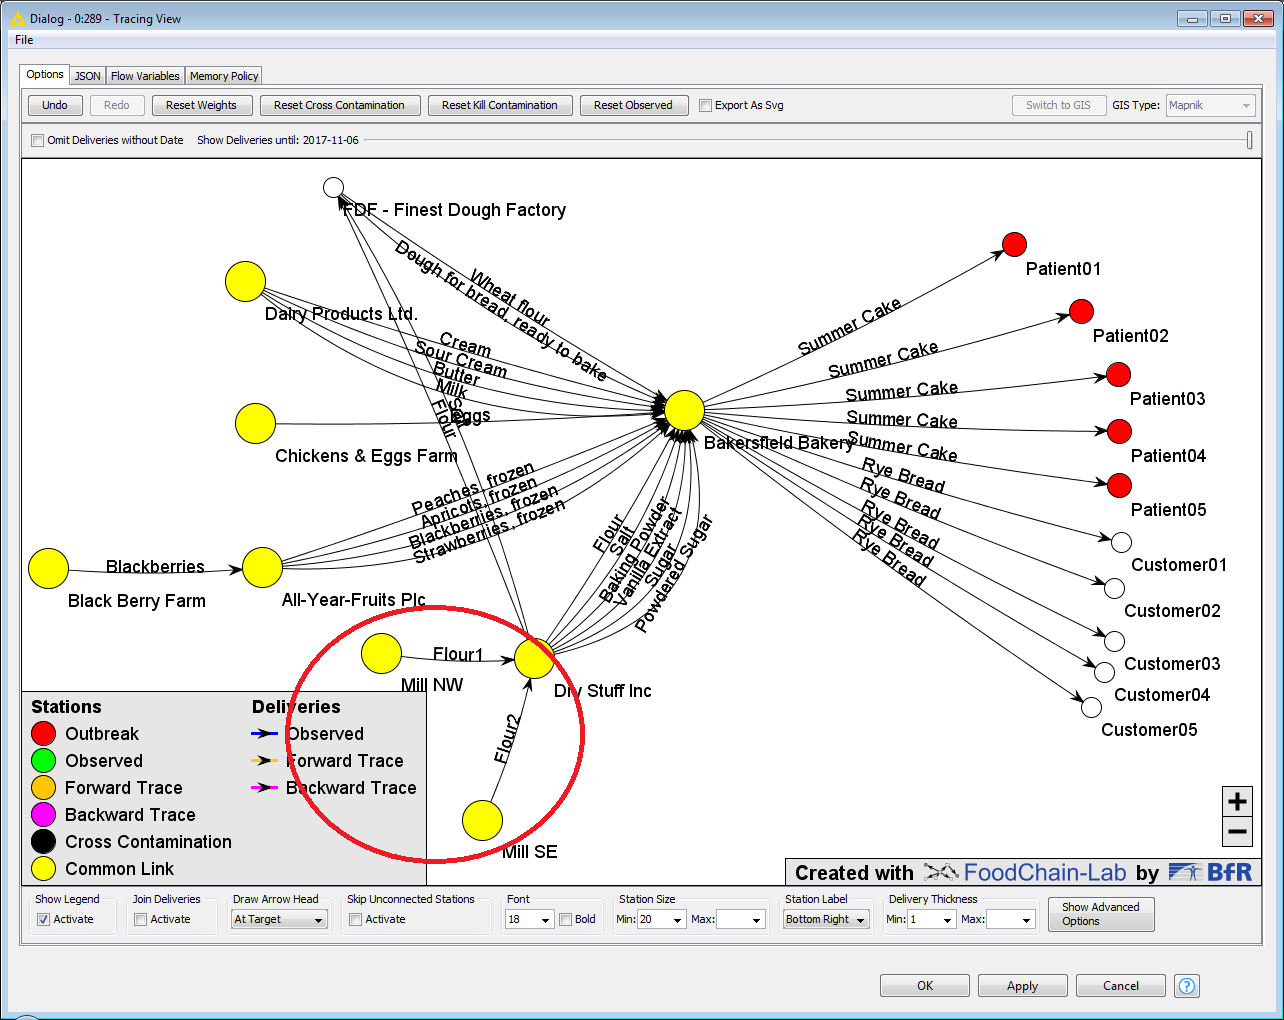
\includegraphics[height=0.6\textheight]{5.png}
	\end{center}
	\begin{itemize}
		\item Reset the \textbf{Supply Chain Reader} and doubleclick the \textbf{Tracing View}. As shown in the above screenshot there should be two new stations (Mill SE and Mill NW) delivering flour to \textit{Dry Stuff Inc}.
	\end{itemize}
\end{frame}

\section{6}
\begin{frame}
	\begin{center}
			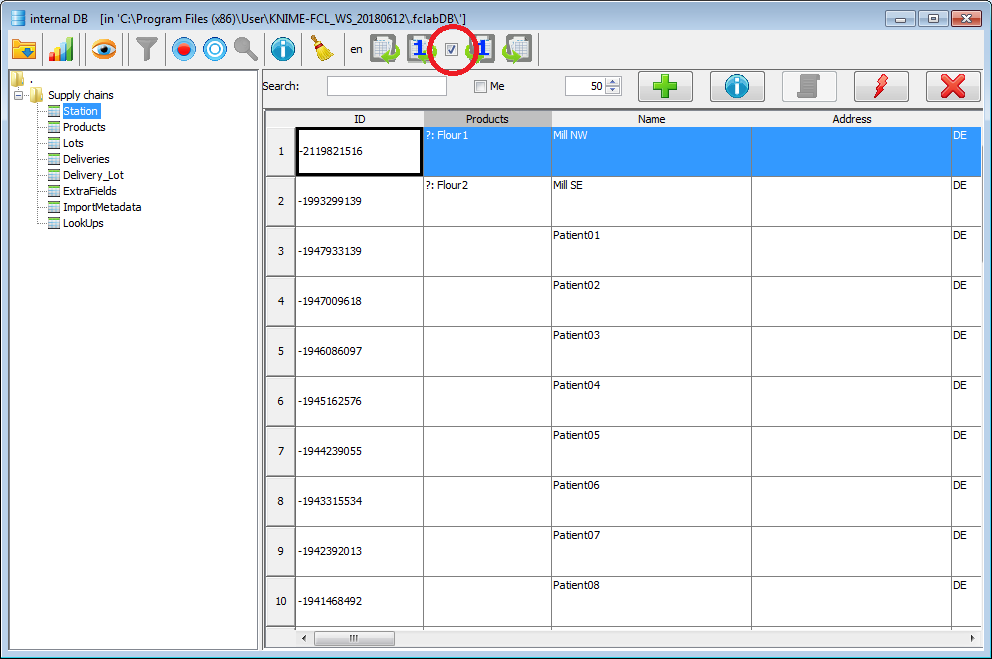
\includegraphics[height=0.6\textheight]{6.png}
	\end{center}
\leftskip1em{Question:}
	\begin{itemize}
		\item What is the difference in the pre-filled Tracing Backward Template if you select or de-select the box ``Generate only missing data''? What could it be useful for?
	\end{itemize}
\end{frame}

\end{document}
